 \documentclass{article}
\usepackage[utf8]{inputenc}
\usepackage[a4paper, total={7in, 10in}]{geometry}
\usepackage{braket}
\usepackage{xcolor}
\usepackage{amsmath}
\usepackage{amssymb}
\usepackage{amsfonts}
\usepackage{graphicx}
\usepackage{svg}
\usepackage{float}
\usepackage{tikz}
\usepackage[ruled,vlined]{algorithm2e}
\usepackage{multicol}
\usepackage[backend=biber,style=alphabetic,sorting=ynt]{biblatex}
\usepackage{xcolor}
%\addbibresource{sample.bib} %Import the bibliography file

\newcommand{\commentt}[1]{\textcolor{blue}{ \textbf{[COMMENT]} #1}}
\newcommand{\ctt}[1]{\commentt{#1}}
\newcommand{\prb}[1]{ \mathbf{Pr} \left[ {#1} \right]}
\newcommand{\onotation}[1]{\(\mathcal{O} \left( {#1}  \right) \)}
\newcommand{\ona}[1]{\onotation{#1}}
\newcommand{\PSI}{{\ket{\psi}}}
\newcommand{\LESn}{\ket{\psi_n}}
\newcommand{\LESa}{\ket{\phi_n}}
\newcommand{\LESs}{\frac{1}{\sqrt{n}}\sum_{i}{\ket{\left(0^{i}10^{n-i}\right)^{n}}}}
\newcommand{\Hn}{\mathcal{H}_{n}}
\newcommand{\Ep}{\frac{1}{\sqrt{2^n}}\sum^{2^n}_{x}{ \ket{xx}}}
\newcommand{\HON}{\ket{\psi_{\text{honest}}}}
\newcommand{\Lemma}{\paragraph{Lemma.}}


\setlength{\columnsep}{0.6cm}

\newcommand{\Gz}{ G_{z}^{\delta} } 

\begin{document}

\title{Quantum LTC With Positive Rate}
\author{David Ponarovsky}
\maketitle
\begin{multicols*}{2}
\newcommand{ \Hw }{ \delta\Delta -\Delta^{\frac{1}{2}-\varepsilon}/\delta  }
	\newcommand{ \Nw }{ \Delta^{\frac{3}{2}-\varepsilon}} 
	  \newcommand{ \Gu } { \Gamma^{\cup} }
	  \newcommand{ \Guq } { \Gamma^{\cup, \square} }

    	\newcommand{ \Gsa } {\Gamma_{\square_{1}} }
	\newcommand{ \Gsb } {\Gamma_{\square_{2}} }
        \newcommand{ \Aa } { C_{A_{1}}}  
	\newcommand{ \Ab } { C_{A_{2}}}
	\newcommand{ \Ac } { C_{A_{3}}}
	\newcommand{ \Aab } { \Aa \otimes \Ab } 
	\newcommand{ \Aac } { \Aa \otimes \Ac }
	\newcommand{ \Aabc } { \Aa \otimes \Ab \otimes \Ac }
	\newcommand{ \Aabp } { \Aa^{\perp} \otimes \Ab^{\perp} } 
	\newcommand{ \Aacp } { \Aa^{\perp} \otimes \Ac^{\perp} }
	\newcommand{ \Aabcp } { \Aa^{\perp} \otimes \Ab^{\perp} \otimes \Ac^{\perp} }
	\newcommand{ \Aabpp } { \left( \Aabp \right)^\perp } 
	\newcommand{ \Aacpp } { \left( \Aacp \right)^\perp }
	\newcommand{ \Aabcpp } { \left( \Aabcp \right)^\perp }
	\newcommand{ \YY } {  y_{1}y_{2}^{\top} }
	\newcommand{ \ZZ } {  z_{1}z_{2}^{\top} } 
	\newcommand{ \TT } { \tilde{\tau} } 


  \paragraph{preamble.} preamble.  
  \begin{figure}[H]
            %\label{fig:square}
            \begin{center}
            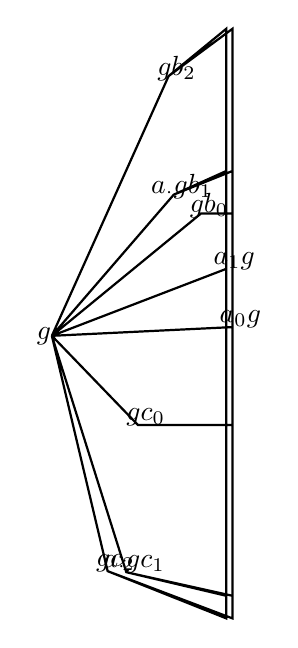
\begin{tikzpicture}
            \draw[thick](0,0)(0,0) -- (1.8957261208379892,1.5547139069053966) -- (2.2936801690819046,1.5547139069053966) -- (2.2936801690819046,0.11081201101858404) -- (0,0)
(0,0) -- (1.5486776675834626,1.7932825956692295) -- (2.2936801690819046,2.0932825956692294) -- (2.2936801690819046,0.11081201101858404) -- (0,0)
(0,0) -- (1.4831156269747863,3.2993747286531447) -- (2.2936801690819046,3.899374728653145) -- (2.2936801690819046,0.11081201101858404) -- (0,0)
(0,0) -- (1.8957261208379892,1.5547139069053966) -- (2.2147895817179046,1.5547139069053966) -- (2.2147895817179046,0.8505139956192503) -- (0,0)
(0,0) -- (1.5486776675834626,1.7932825956692295) -- (2.2147895817179046,2.0932825956692294) -- (2.2147895817179046,0.8505139956192503) -- (0,0)
(0,0) -- (1.4831156269747863,3.2993747286531447) -- (2.2147895817179046,3.899374728653145) -- (2.2147895817179046,0.8505139956192503) -- (0,0)
(0,0) -- (1.0921408115922768,-1.131336188926464) -- (2.2936801690819046,-1.131336188926464) -- (2.2936801690819046,0.11081201101858404) -- (0,0)
(0,0) -- (0.9451530738502221,-3.0016507773300676) -- (2.2936801690819046,-3.3016507773300674) -- (2.2936801690819046,0.11081201101858404) -- (0,0)
(0,0) -- (0.7082312383158864,-2.9884620512959756) -- (2.2936801690819046,-3.5884620512959757) -- (2.2936801690819046,0.11081201101858404) -- (0,0)
(0,0) -- (1.0921408115922768,-1.131336188926464) -- (2.2147895817179046,-1.131336188926464) -- (2.2147895817179046,0.8505139956192503) -- (0,0)
(0,0) -- (0.9451530738502221,-3.0016507773300676) -- (2.2147895817179046,-3.3016507773300674) -- (2.2147895817179046,0.8505139956192503) -- (0,0)
(0,0) -- (0.7082312383158864,-2.9884620512959756) -- (2.2147895817179046,-3.5884620512959757) -- (2.2147895817179046,0.8505139956192503) -- (0,0)
;
\node at (-0.1,0) {$ g $};
\node at (2.3936801690819047,0.21081201101858404) {$ a_{ 0 }g $};
\node at (2.3147895817179047,0.9505139956192503) {$ a_{ 1 }g $};
\node at (1.9957261208379893,1.6547139069053967) {$ gb_{ 0 } $};
\node at (1.6486776675834627,1.8932825956692296) {$ a_{\cdot} gb_{ 1 } $};
\node at (1.5831156269747864,3.399374728653145) {$ gb_{ 2 } $};
\node at (1.192140811592277,-1.0313361889264638) {$ gc_{ 0 } $};
\node at (1.0451530738502222,-2.9016507773300675) {$ a_{\cdot} gc_{ 1 } $};
\node at (0.8082312383158864,-2.8884620512959756) {$ gc_{ 2 } $};

            \end{tikzpicture}
            \end{center}
            \caption{Square of the complex, with edges $(g,ag), (agb, gb) \in E_A,
            (g,gb), (agb, ag) \in E_B.$ \label{fig:square}
            }
            \end{figure}
 \begin{figure}[H]
            %\label{fig:square}
            \begin{center}
            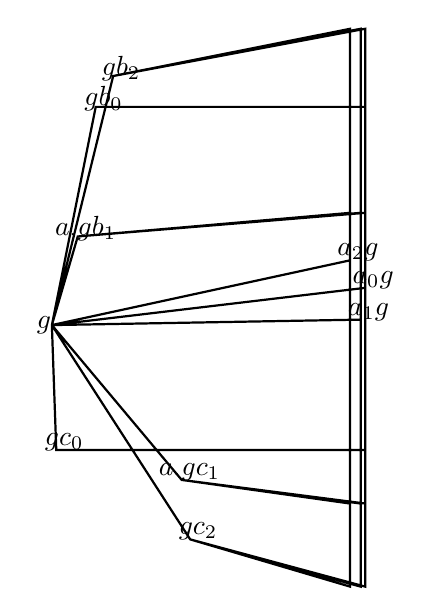
\begin{tikzpicture}
            \draw[thick](0,0)(0,0) -- (0.5568910158509275,2.771160969551166) -- (3.980010601959853,2.771160969551166) -- (3.980010601959853,0.47293669654829007) -- (0,0)
(0,0) -- (0.32887481349855774,1.1254876202735673) -- (3.980010601959853,1.4254876202735673) -- (3.980010601959853,0.47293669654829007) -- (0,0)
(0,0) -- (0.7787118589370559,3.1630233596124295) -- (3.980010601959853,3.7630233596124296) -- (3.980010601959853,0.47293669654829007) -- (0,0)
(0,0) -- (0.5568910158509275,2.771160969551166) -- (3.9215051814575004,2.771160969551166) -- (3.9215051814575004,0.06927673696166016) -- (0,0)
(0,0) -- (0.32887481349855774,1.1254876202735673) -- (3.9215051814575004,1.4254876202735673) -- (3.9215051814575004,0.06927673696166016) -- (0,0)
(0,0) -- (0.7787118589370559,3.1630233596124295) -- (3.9215051814575004,3.7630233596124296) -- (3.9215051814575004,0.06927673696166016) -- (0,0)
(0,0) -- (0.5568910158509275,2.771160969551166) -- (3.7875478231962703,2.771160969551166) -- (3.7875478231962703,0.822416740533561) -- (0,0)
(0,0) -- (0.32887481349855774,1.1254876202735673) -- (3.7875478231962703,1.4254876202735673) -- (3.7875478231962703,0.822416740533561) -- (0,0)
(0,0) -- (0.7787118589370559,3.1630233596124295) -- (3.7875478231962703,3.7630233596124296) -- (3.7875478231962703,0.822416740533561) -- (0,0)
(0,0) -- (0.05587479312671739,-1.5858342855927288) -- (3.980010601959853,-1.5858342855927288) -- (3.980010601959853,0.47293669654829007) -- (0,0)
(0,0) -- (1.6487558703623784,-1.966445538354309) -- (3.980010601959853,-2.2664455383543087) -- (3.980010601959853,0.47293669654829007) -- (0,0)
(0,0) -- (1.7567930147694173,-2.72160236579034) -- (3.980010601959853,-3.32160236579034) -- (3.980010601959853,0.47293669654829007) -- (0,0)
(0,0) -- (0.05587479312671739,-1.5858342855927288) -- (3.9215051814575004,-1.5858342855927288) -- (3.9215051814575004,0.06927673696166016) -- (0,0)
(0,0) -- (1.6487558703623784,-1.966445538354309) -- (3.9215051814575004,-2.2664455383543087) -- (3.9215051814575004,0.06927673696166016) -- (0,0)
(0,0) -- (1.7567930147694173,-2.72160236579034) -- (3.9215051814575004,-3.32160236579034) -- (3.9215051814575004,0.06927673696166016) -- (0,0)
(0,0) -- (0.05587479312671739,-1.5858342855927288) -- (3.7875478231962703,-1.5858342855927288) -- (3.7875478231962703,0.822416740533561) -- (0,0)
(0,0) -- (1.6487558703623784,-1.966445538354309) -- (3.7875478231962703,-2.2664455383543087) -- (3.7875478231962703,0.822416740533561) -- (0,0)
(0,0) -- (1.7567930147694173,-2.72160236579034) -- (3.7875478231962703,-3.32160236579034) -- (3.7875478231962703,0.822416740533561) -- (0,0)
;
\node at (-0.1,0) {$ g $};
\node at (4.080010601959853,0.57293669654829) {$ a_{ 0 }g $};
\node at (4.0215051814575,0.16927673696166018) {$ a_{ 1 }g $};
\node at (3.8875478231962703,0.9224167405335609) {$ a_{ 2 }g $};
\node at (0.6568910158509275,2.871160969551166) {$ gb_{ 0 } $};
\node at (0.4288748134985577,1.2254876202735674) {$ a_{\cdot} gb_{ 1 } $};
\node at (0.8787118589370558,3.2630233596124296) {$ gb_{ 2 } $};
\node at (0.1558747931267174,-1.4858342855927287) {$ gc_{ 0 } $};
\node at (1.7487558703623785,-1.8664455383543088) {$ a_{\cdot} gc_{ 1 } $};
\node at (1.8567930147694174,-2.62160236579034) {$ gc_{ 2 } $};

            \end{tikzpicture}
            \end{center}
            \caption{Square of the complex, with edges $(g,ag), (agb, gb) \in E_A,
            (g,gb), (agb, ag) \in E_B.$ \label{fig:square}
            }
            \end{figure}
 \begin{figure}[H]
            %\label{fig:square}
            \begin{center}
            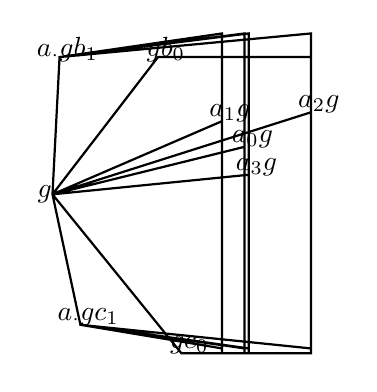
\begin{tikzpicture}
            \draw[thick](0,0)(0,0) -- (1.340167167028735,1.742837199492465) -- (2.4391188889798103,1.742837199492465) -- (2.4391188889798103,0.6032986220046778) -- (0,0)
(0,0) -- (0.08994976277748257,1.7432011640167482) -- (2.4391188889798103,2.043201164016748) -- (2.4391188889798103,0.6032986220046778) -- (0,0)
(0,0) -- (1.340167167028735,1.742837199492465) -- (2.153779186419458,1.742837199492465) -- (2.153779186419458,0.9294433794103998) -- (0,0)
(0,0) -- (0.08994976277748257,1.7432011640167482) -- (2.153779186419458,2.043201164016748) -- (2.153779186419458,0.9294433794103998) -- (0,0)
(0,0) -- (1.340167167028735,1.742837199492465) -- (3.2827963532942395,1.742837199492465) -- (3.2827963532942395,1.0418323731276211) -- (0,0)
(0,0) -- (0.08994976277748257,1.7432011640167482) -- (3.2827963532942395,2.043201164016748) -- (3.2827963532942395,1.0418323731276211) -- (0,0)
(0,0) -- (1.340167167028735,1.742837199492465) -- (2.4915661863819447,1.742837199492465) -- (2.4915661863819447,0.2485017447176022) -- (0,0)
(0,0) -- (0.08994976277748257,1.7432011640167482) -- (2.4915661863819447,2.043201164016748) -- (2.4915661863819447,0.2485017447176022) -- (0,0)
(0,0) -- (1.6381876363587267,-2.019615037539465) -- (2.4391188889798103,-2.019615037539465) -- (2.4391188889798103,0.6032986220046778) -- (0,0)
(0,0) -- (0.35479439376560284,-1.657024303114513) -- (2.4391188889798103,-1.9570243031145131) -- (2.4391188889798103,0.6032986220046778) -- (0,0)
(0,0) -- (1.6381876363587267,-2.019615037539465) -- (2.153779186419458,-2.019615037539465) -- (2.153779186419458,0.9294433794103998) -- (0,0)
(0,0) -- (0.35479439376560284,-1.657024303114513) -- (2.153779186419458,-1.9570243031145131) -- (2.153779186419458,0.9294433794103998) -- (0,0)
(0,0) -- (1.6381876363587267,-2.019615037539465) -- (3.2827963532942395,-2.019615037539465) -- (3.2827963532942395,1.0418323731276211) -- (0,0)
(0,0) -- (0.35479439376560284,-1.657024303114513) -- (3.2827963532942395,-1.9570243031145131) -- (3.2827963532942395,1.0418323731276211) -- (0,0)
(0,0) -- (1.6381876363587267,-2.019615037539465) -- (2.4915661863819447,-2.019615037539465) -- (2.4915661863819447,0.2485017447176022) -- (0,0)
(0,0) -- (0.35479439376560284,-1.657024303114513) -- (2.4915661863819447,-1.9570243031145131) -- (2.4915661863819447,0.2485017447176022) -- (0,0)
;
\node at (-0.1,0) {$ g $};
\node at (2.5391188889798104,0.7032986220046777) {$ a_{ 0 }g $};
\node at (2.2537791864194583,1.0294433794103999) {$ a_{ 1 }g $};
\node at (3.3827963532942396,1.1418323731276212) {$ a_{ 2 }g $};
\node at (2.591566186381945,0.3485017447176022) {$ a_{ 3 }g $};
\node at (1.440167167028735,1.842837199492465) {$ gb_{ 0 } $};
\node at (0.18994976277748257,1.8432011640167483) {$ a_{\cdot} gb_{ 1 } $};
\node at (1.7381876363587268,-1.9196150375394647) {$ gc_{ 0 } $};
\node at (0.4547943937656028,-1.557024303114513) {$ a_{\cdot} gc_{ 1 } $};

            \end{tikzpicture}
            \end{center}
            \caption{Square of the complex, with edges $(g,ag), (agb, gb) \in E_A,
            (g,gb), (agb, ag) \in E_B.$ \label{fig:square}
            }
            \end{figure}
 \begin{figure}[H]
            %\label{fig:square}
            \begin{center}
            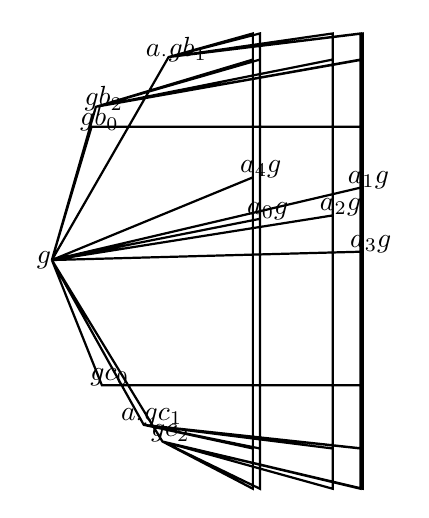
\begin{tikzpicture}
            \draw[thick](0,0)(0,0) -- (0.5041216186077406,1.6917267473030937) -- (2.6424904119800043,1.6917267473030937) -- (2.6424904119800043,0.5233170352704232) -- (0,0)
(0,0) -- (1.4823945306067154,2.5776465532008834) -- (2.6424904119800043,2.8776465532008833) -- (2.6424904119800043,0.5233170352704232) -- (0,0)
(0,0) -- (0.5590402242522738,1.9459550780980974) -- (2.6424904119800043,2.5459550780980975) -- (2.6424904119800043,0.5233170352704232) -- (0,0)
(0,0) -- (0.5041216186077406,1.6917267473030937) -- (3.9199628673301627,1.6917267473030937) -- (3.9199628673301627,0.9193525104689905) -- (0,0)
(0,0) -- (1.4823945306067154,2.5776465532008834) -- (3.9199628673301627,2.8776465532008833) -- (3.9199628673301627,0.9193525104689905) -- (0,0)
(0,0) -- (0.5590402242522738,1.9459550780980974) -- (3.9199628673301627,2.5459550780980975) -- (3.9199628673301627,0.9193525104689905) -- (0,0)
(0,0) -- (0.5041216186077406,1.6917267473030937) -- (3.5669777744512263,1.6917267473030937) -- (3.5669777744512263,0.5666516163012236) -- (0,0)
(0,0) -- (1.4823945306067154,2.5776465532008834) -- (3.5669777744512263,2.8776465532008833) -- (3.5669777744512263,0.5666516163012236) -- (0,0)
(0,0) -- (0.5590402242522738,1.9459550780980974) -- (3.5669777744512263,2.5459550780980975) -- (3.5669777744512263,0.5666516163012236) -- (0,0)
(0,0) -- (0.5041216186077406,1.6917267473030937) -- (3.9497139303341386,1.6917267473030937) -- (3.9497139303341386,0.10637556815729678) -- (0,0)
(0,0) -- (1.4823945306067154,2.5776465532008834) -- (3.9497139303341386,2.8776465532008833) -- (3.9497139303341386,0.10637556815729678) -- (0,0)
(0,0) -- (0.5590402242522738,1.9459550780980974) -- (3.9497139303341386,2.5459550780980975) -- (3.9497139303341386,0.10637556815729678) -- (0,0)
(0,0) -- (0.5041216186077406,1.6917267473030937) -- (2.5527414116488725,1.6917267473030937) -- (2.5527414116488725,1.0501650164934917) -- (0,0)
(0,0) -- (1.4823945306067154,2.5776465532008834) -- (2.5527414116488725,2.8776465532008833) -- (2.5527414116488725,1.0501650164934917) -- (0,0)
(0,0) -- (0.5590402242522738,1.9459550780980974) -- (2.5527414116488725,2.5459550780980975) -- (2.5527414116488725,1.0501650164934917) -- (0,0)
(0,0) -- (0.6352777902095401,-1.5898836683067166) -- (2.6424904119800043,-1.5898836683067166) -- (2.6424904119800043,0.5233170352704232) -- (0,0)
(0,0) -- (1.167377371797261,-2.093490079848137) -- (2.6424904119800043,-2.393490079848137) -- (2.6424904119800043,0.5233170352704232) -- (0,0)
(0,0) -- (1.4043677519788405,-2.30486319703041) -- (2.6424904119800043,-2.90486319703041) -- (2.6424904119800043,0.5233170352704232) -- (0,0)
(0,0) -- (0.6352777902095401,-1.5898836683067166) -- (3.9199628673301627,-1.5898836683067166) -- (3.9199628673301627,0.9193525104689905) -- (0,0)
(0,0) -- (1.167377371797261,-2.093490079848137) -- (3.9199628673301627,-2.393490079848137) -- (3.9199628673301627,0.9193525104689905) -- (0,0)
(0,0) -- (1.4043677519788405,-2.30486319703041) -- (3.9199628673301627,-2.90486319703041) -- (3.9199628673301627,0.9193525104689905) -- (0,0)
(0,0) -- (0.6352777902095401,-1.5898836683067166) -- (3.5669777744512263,-1.5898836683067166) -- (3.5669777744512263,0.5666516163012236) -- (0,0)
(0,0) -- (1.167377371797261,-2.093490079848137) -- (3.5669777744512263,-2.393490079848137) -- (3.5669777744512263,0.5666516163012236) -- (0,0)
(0,0) -- (1.4043677519788405,-2.30486319703041) -- (3.5669777744512263,-2.90486319703041) -- (3.5669777744512263,0.5666516163012236) -- (0,0)
(0,0) -- (0.6352777902095401,-1.5898836683067166) -- (3.9497139303341386,-1.5898836683067166) -- (3.9497139303341386,0.10637556815729678) -- (0,0)
(0,0) -- (1.167377371797261,-2.093490079848137) -- (3.9497139303341386,-2.393490079848137) -- (3.9497139303341386,0.10637556815729678) -- (0,0)
(0,0) -- (1.4043677519788405,-2.30486319703041) -- (3.9497139303341386,-2.90486319703041) -- (3.9497139303341386,0.10637556815729678) -- (0,0)
(0,0) -- (0.6352777902095401,-1.5898836683067166) -- (2.5527414116488725,-1.5898836683067166) -- (2.5527414116488725,1.0501650164934917) -- (0,0)
(0,0) -- (1.167377371797261,-2.093490079848137) -- (2.5527414116488725,-2.393490079848137) -- (2.5527414116488725,1.0501650164934917) -- (0,0)
(0,0) -- (1.4043677519788405,-2.30486319703041) -- (2.5527414116488725,-2.90486319703041) -- (2.5527414116488725,1.0501650164934917) -- (0,0)
;
\node at (-0.1,0) {$ g $};
\node at (2.7424904119800044,0.6233170352704231) {$ a_{ 0 }g $};
\node at (4.019962867330163,1.0193525104689904) {$ a_{ 1 }g $};
\node at (3.6669777744512264,0.6666516163012236) {$ a_{ 2 }g $};
\node at (4.049713930334138,0.2063755681572968) {$ a_{ 3 }g $};
\node at (2.6527414116488726,1.1501650164934918) {$ a_{ 4 }g $};
\node at (0.6041216186077406,1.7917267473030938) {$ gb_{ 0 } $};
\node at (1.5823945306067155,2.6776465532008835) {$ a_{\cdot} gb_{ 1 } $};
\node at (0.6590402242522738,2.0459550780980975) {$ gb_{ 2 } $};
\node at (0.7352777902095401,-1.4898836683067165) {$ gc_{ 0 } $};
\node at (1.2673773717972612,-1.993490079848137) {$ a_{\cdot} gc_{ 1 } $};
\node at (1.5043677519788405,-2.20486319703041) {$ gc_{ 2 } $};

            \end{tikzpicture}
            \end{center}
            \caption{Square of the complex, with edges $(g,ag), (agb, gb) \in E_A,
            (g,gb), (agb, ag) \in E_B.$ \label{fig:square}
            }
            \end{figure}
 \begin{figure}[H]
            %\label{fig:square}
            \begin{center}
            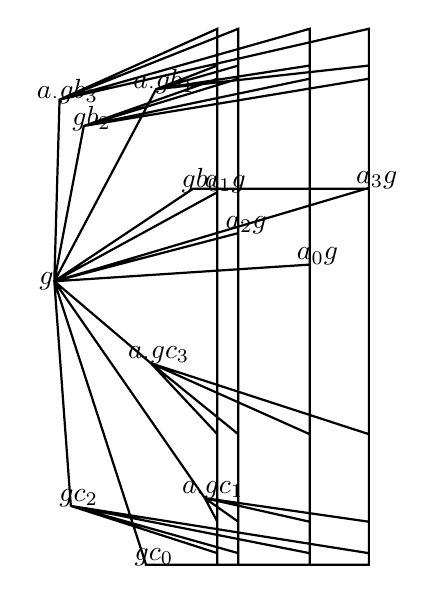
\begin{tikzpicture}
            \draw[thick](0,0)(0,0) -- (1.7618541612285255,1.1751413817945329) -- (3.2431605620675468,1.1751413817945329) -- (3.2431605620675468,0.21175543766092) -- (0,0)
(0,0) -- (1.292038428874793,2.4394831095322314) -- (3.2431605620675468,2.739483109532231) -- (3.2431605620675468,0.21175543766092) -- (0,0)
(0,0) -- (0.3740732898392518,1.9722462484288974) -- (3.2431605620675468,2.5722462484288973) -- (3.2431605620675468,0.21175543766092) -- (0,0)
(0,0) -- (0.06645787663651204,2.306722261580971) -- (3.2431605620675468,3.2067222615809707) -- (3.2431605620675468,0.21175543766092) -- (0,0)
(0,0) -- (1.7618541612285255,1.1751413817945329) -- (2.0704681970697476,1.1751413817945329) -- (2.0704681970697476,1.1311692410853218) -- (0,0)
(0,0) -- (1.292038428874793,2.4394831095322314) -- (2.0704681970697476,2.739483109532231) -- (2.0704681970697476,1.1311692410853218) -- (0,0)
(0,0) -- (0.3740732898392518,1.9722462484288974) -- (2.0704681970697476,2.5722462484288973) -- (2.0704681970697476,1.1311692410853218) -- (0,0)
(0,0) -- (0.06645787663651204,2.306722261580971) -- (2.0704681970697476,3.2067222615809707) -- (2.0704681970697476,1.1311692410853218) -- (0,0)
(0,0) -- (1.7618541612285255,1.1751413817945329) -- (2.336255182152895,1.1751413817945329) -- (2.336255182152895,0.6121716026093781) -- (0,0)
(0,0) -- (1.292038428874793,2.4394831095322314) -- (2.336255182152895,2.739483109532231) -- (2.336255182152895,0.6121716026093781) -- (0,0)
(0,0) -- (0.3740732898392518,1.9722462484288974) -- (2.336255182152895,2.5722462484288973) -- (2.336255182152895,0.6121716026093781) -- (0,0)
(0,0) -- (0.06645787663651204,2.306722261580971) -- (2.336255182152895,3.2067222615809707) -- (2.336255182152895,0.6121716026093781) -- (0,0)
(0,0) -- (1.7618541612285255,1.1751413817945329) -- (3.994769808584086,1.1751413817945329) -- (3.994769808584086,1.1857821364812882) -- (0,0)
(0,0) -- (1.292038428874793,2.4394831095322314) -- (3.994769808584086,2.739483109532231) -- (3.994769808584086,1.1857821364812882) -- (0,0)
(0,0) -- (0.3740732898392518,1.9722462484288974) -- (3.994769808584086,2.5722462484288973) -- (3.994769808584086,1.1857821364812882) -- (0,0)
(0,0) -- (0.06645787663651204,2.306722261580971) -- (3.994769808584086,3.2067222615809707) -- (3.994769808584086,1.1857821364812882) -- (0,0)
(0,0) -- (1.1654471358030765,-3.6008455797253216) -- (3.2431605620675468,-3.6008455797253216) -- (3.2431605620675468,0.21175543766092) -- (0,0)
(0,0) -- (1.9109537841652378,-2.7537158449764907) -- (3.2431605620675468,-3.0537158449764905) -- (3.2431605620675468,0.21175543766092) -- (0,0)
(0,0) -- (0.20976586923644147,-2.852975669928725) -- (3.2431605620675468,-3.4529756699287253) -- (3.2431605620675468,0.21175543766092) -- (0,0)
(0,0) -- (1.2271818375993226,-1.0419298472121792) -- (3.2431605620675468,-1.941929847212179) -- (3.2431605620675468,0.21175543766092) -- (0,0)
(0,0) -- (1.1654471358030765,-3.6008455797253216) -- (2.0704681970697476,-3.6008455797253216) -- (2.0704681970697476,1.1311692410853218) -- (0,0)
(0,0) -- (1.9109537841652378,-2.7537158449764907) -- (2.0704681970697476,-3.0537158449764905) -- (2.0704681970697476,1.1311692410853218) -- (0,0)
(0,0) -- (0.20976586923644147,-2.852975669928725) -- (2.0704681970697476,-3.4529756699287253) -- (2.0704681970697476,1.1311692410853218) -- (0,0)
(0,0) -- (1.2271818375993226,-1.0419298472121792) -- (2.0704681970697476,-1.941929847212179) -- (2.0704681970697476,1.1311692410853218) -- (0,0)
(0,0) -- (1.1654471358030765,-3.6008455797253216) -- (2.336255182152895,-3.6008455797253216) -- (2.336255182152895,0.6121716026093781) -- (0,0)
(0,0) -- (1.9109537841652378,-2.7537158449764907) -- (2.336255182152895,-3.0537158449764905) -- (2.336255182152895,0.6121716026093781) -- (0,0)
(0,0) -- (0.20976586923644147,-2.852975669928725) -- (2.336255182152895,-3.4529756699287253) -- (2.336255182152895,0.6121716026093781) -- (0,0)
(0,0) -- (1.2271818375993226,-1.0419298472121792) -- (2.336255182152895,-1.941929847212179) -- (2.336255182152895,0.6121716026093781) -- (0,0)
(0,0) -- (1.1654471358030765,-3.6008455797253216) -- (3.994769808584086,-3.6008455797253216) -- (3.994769808584086,1.1857821364812882) -- (0,0)
(0,0) -- (1.9109537841652378,-2.7537158449764907) -- (3.994769808584086,-3.0537158449764905) -- (3.994769808584086,1.1857821364812882) -- (0,0)
(0,0) -- (0.20976586923644147,-2.852975669928725) -- (3.994769808584086,-3.4529756699287253) -- (3.994769808584086,1.1857821364812882) -- (0,0)
(0,0) -- (1.2271818375993226,-1.0419298472121792) -- (3.994769808584086,-1.941929847212179) -- (3.994769808584086,1.1857821364812882) -- (0,0)
;
\node at (-0.1,0) {$ g $};
\node at (3.343160562067547,0.31175543766092) {$ a_{ 0 }g $};
\node at (2.1704681970697477,1.2311692410853219) {$ a_{ 1 }g $};
\node at (2.436255182152895,0.7121716026093781) {$ a_{ 2 }g $};
\node at (4.094769808584086,1.2857821364812883) {$ a_{ 3 }g $};
\node at (1.8618541612285255,1.275141381794533) {$ gb_{ 0 } $};
\node at (1.3920384288747931,2.5394831095322314) {$ a_{\cdot} gb_{ 1 } $};
\node at (0.4740732898392518,2.0722462484288973) {$ gb_{ 2 } $};
\node at (0.16645787663651204,2.406722261580971) {$ a_{\cdot} gb_{ 3 } $};
\node at (1.2654471358030766,-3.5008455797253215) {$ gc_{ 0 } $};
\node at (2.010953784165238,-2.6537158449764906) {$ a_{\cdot} gc_{ 1 } $};
\node at (0.30976586923644145,-2.752975669928725) {$ gc_{ 2 } $};
\node at (1.3271818375993227,-0.9419298472121792) {$ a_{\cdot} gc_{ 3 } $};

            \end{tikzpicture}
            \end{center}
            \caption{Square of the complex, with edges $(g,ag), (agb, gb) \in E_A,
            (g,gb), (agb, ag) \in E_B.$ \label{fig:square}
            }
            \end{figure}
 
\end{multicols*}
  % \printbibliography 
\end{document}

 